\chapter{Rekonstrukcja śladów}

Rozdział ten ma na celu przedstawienie procesu rekonstrukcji śladów w eksperymencie LHCb. Na samym początku, pokrótce omówione będą oddziaływania cząstek z materią, następnie autor skupia się na opisaniu strategii znajdowania śladów. 

Rekonstrukcja śladów jest procedurą wykonywaną w celu znalezienie trajektorii lotu naładowanej cząstki przez detektor. Jest to niezbędny punkt praktycznie każdego eksperymentu z dziedziny fizyki cząstek elementarnych, głównym celem wykonywania tej skomplikowanej procedury jest pomiar wartości trzech składowych pędu cząstki. 

\section{Oddziaływanie cząstek z materią}
Kiedy cząstka przechodzi przez materię oddziałuje z nią. Istnieją dwa typy oddziaływań: elektromagnetyczne oraz hadronowe\footnote{W ogólności występują jeszcze oddziaływania słabe, lecz nie są one istotne z punktu widzenia znajdowania śladów}. 
\subsection{Oddziaływania elektromagnetyczne}
Możliwe są następujące typy oddziaływań elektromagnetycznych:
\begin{itemize}
\item \textbf{Jonizacja} zachodzi gdy naładowana cząstka podróżując przez materiał wzbudza atom do wyższego stanu, lub gdy jonizuje go przez oddziaływanie z zewnętrznym elektronem. Średnia wartość traconej energii jest opisana pół-empirycznym wzorem Bethego-Blocha\cite{Bete}: 
\begin{equation}
-\left< \frac{dE}{dx} \right> = Kz^2\frac{Z}{A}\frac{1}{\beta^2}\left[\frac{1}{2}log\left(\frac{2m_ec^2\beta^2\gamma^2T_{max}}{I^2}\right) -\beta^2-\frac{\delta(\beta\gamma)}{2} \right]
\label{bethe}
\end{equation}
gdzie: \\
$K=\frac{4\pi e^2}{c^2m_e}N_A$, przy czym $e$ ładunek elementarny, $c$ prędkość światła, $m_e$ masa elektronu, $N_A$ stałą Avogadro, $z$ ładunek cząstki ( w jednostkach ładunku elementarnego), $Z$ liczba atomowa absorbentu, $A$ liczba masowa absorbentu, $\beta=\frac{v}{c}$, $I$ średnia energia jonizacji (w eV), $T_{max}$ maksymalna energia kinetyczna przekazywana do swobodnego elektronu w pojedynczym zderzeniu, $\delta(\beta\gamma)$ poprawka do energii wynikająca z elektrostatycznej polaryzacji ośrodka.

Warto zwrócić uwagę, że formuła Bethego-Blocha opisuje średnią energię traconą w przedziale prędkości $0.1<\beta\gamma<1000$ z precyzją kilku procent. Z powyższego równania można wywnioskować, że najbardziej istotnymi przyczynkami do straty energii cząstki poprzez jonizację pochodzą od prędkości cząstki, jej ładunku i gęstości materiału.

\item \textbf{Rozpraszanie Coulombowskie}, również zwane rozpraszanie Rutherforda, ten typ oddziaływania występuje pomiędzy cząstkami oraz jądrami atomowymi w materiale. W przeciwieństwie do wcześniej opisanej jonizacji zjawisko to nie prowadzi do strat energii, tyko do zmiany trajektorii lotu cząstki. Poza pojedynczym rozproszeniem Coulomba często zachodzi zwielokrotnienie tego procesu tzw. \textbf{wielokrotnego rozpraszania Coulomba}.

\item \textbf{Bremsstrahlung} zachodzi, gdy naładowana cząstka emituje foton pod wpływem pola pochodzącego od jąder atomowych. Jest to dominujący sposób na stratę energii elektronu w eksperymentach Fizyki Wysokich Energii.
\end{itemize}
\subsection{Oddziaływania hadronowe}
W wyniku oddziaływań hadronowych, hadrony powodują niszczenie jąder atomowych, co prowadzi do uwalniania protonów oraz neutronów (proces ten nazywa się spalacją) lub też prowadzi do głębokiego nieelastycznego rozpraszania, które to produkuje nowe hadrony, w większości piony. 
Cząstka oddziałująca hadronowo jest często tracona i dalsze jej śledzenie nie jest już możliwe. Przekrój czynny zależy od typu cząstki, jej ładunku oraz pędu. 

\section{Algorytm rekonstrukcji śladów}
\subsection{Parametryzacja śladów}
Cząstka podróżując przez układ detektorów śladowych oznacza w miejscach oddziaływania punkty. Punkty te zwane potocznie z angielskiego \textit{hitami}. Zbiór takich punktów można wykorzystać do zrekonstruowania ścieżki, po której oryginalnie poruszała się cząstka poprzez dopasowanie odpowiedniej trajektorii ruchu.  Znalezienie tej trajektorii jest niezbędne aby dokonać pomiaru pędu cząstki. Zrekonstruowany ślad (ang. track) jest przechowywany jako zbiór tzw. stanów (ang. states). W praktycznym zastosowaniu stan jest prostą styczną do trajektorii w określonym punkcie o współrzędnej $z$. Tak zdefiniowany stan $\vec{x}_z$ może zostać sparametryzowany przy użyciu: 
\begin{equation}
\vec{x}_z=\begin{pmatrix}
x\\ y \\ t_x \\ t_y \\ \frac{q}{p}
\end{pmatrix}
\end{equation}
gdzie: $x,y,z$ są składowymi kartezjańskimi zależnymi od punktu oddziaływania, przy czym oś $z$ skierowana tak, aby wskazywać oś wiązki,  natomiast oś $y$ jest skierowana zgodnie z kierunkiem pola magnetycznego. Wartości $t_x=\frac{dx}{dz}$ oraz $t_y=\frac{dy}{dz}$ są nachyleniami ścieżki. Ostatni parametr $\frac{q}{p}$ jest ładunkiem podzielonym przez wartość pędu. Warto zwrócić uwagę, że przyjmuje się $q= \pm 1$.

Poza samymi wartościami parametrów opisujących ślady kluczowa jest macierz kowariancji pomiędzy nimi.

\subsection{Typy śladów}
\ref{typySladow}
LHCb używa pięć głównych kategorii śladów, co zostało zaprezentowana na schemacie z rysunku \ref{slady}. Poniżej przedstawiono wyjaśnienie nazw typów śladów.
\begin{figure}[h]
  \centering
  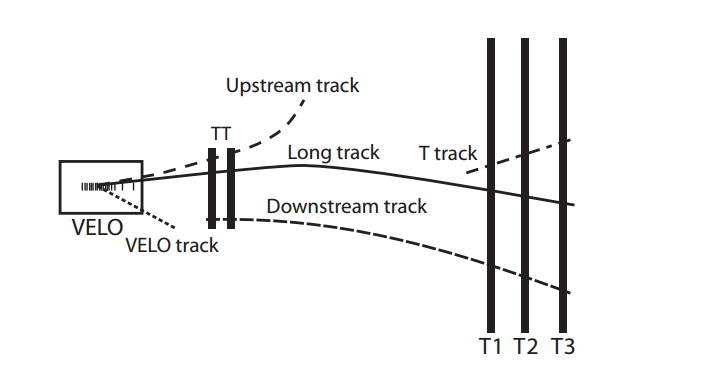
\includegraphics[scale=0.7]{rozdzial3/tracks.png}
  % AccComple.gif: 480x434 pixel, 72dpi, 16.93x15.31 cm, bb=0 0 480 434
  \caption{Poglądowym rysunek śladów w LHCb \cite{trackDefinition}}
  \label{slady}
\end{figure}
  
\begin{itemize}
\item \textbf{Ślady długie} (ang. long tracks) zawierają informacje ze wszystkich detektorów śladowych zainstalowanych w LHCb, co czyni je optymalne z punktu widzenia fizycznych analiz. Oszacowanie pędą na ich podstawie jest najbardziej dokładne. das
\item \textbf{Ślady Velo} zawierają tylko pomiary z detektora Velo w rezultacie czego nie dostarczają żadnej informacji o pędzie cząstki. Natomiast mogą być użyte np. w celu znalezienia wierzchołka pierwotnego. 
\item \textbf{Ślady upstream} są to ślady składające się z pomiarów dokonanych zarówno przez Velo jak i TT, natomiast nie zawierają informacji ze stacji TT. Dzieje się tak w przypadkach, kiedy cząstka wypada z obszaru akceptanci detektorów T.   
\item \textbf{Ślady downstream} bazują na pomiarach tylko w detektorach TT oraz stacjach T. Są wykorzystywane do rekonstrukcji neutralnych cząstek rozpadających się poza obszarem Velo. 
\item \textbf{Ślady T}  zawierają tylko informacje ze stacji T. Taki ślad może zostać wykorzystany np. w algorytmie rozpoznawania wzorców dla detektora RICH2. 
\end{itemize}
\subsection{Rozpoznawania wzorców}
Pierwszym etapem w procesie rekonstrukcji śladów jest algorytm rozpoznawania wzorców, który to rozpoczyna pracę od budowy segmentów śladów w detektorach VELO oraz stacjach T. Tak powstałe zalążki śladów są następnie rozszerzane. Do wykonania powierzonego zadania w eksperymencie LHCb zaimplementowany kilka typów algorytmów rozpoznających wzorce, których celem jest znjdowanie śladów opisanych w podrozdziale \ref{typySladow}. Poniżej znajduje się skrótowy opis każdego z nich. 

\begin{itemize}
\item \textbf{Zalążki śladów VELO} Klastry zmierzone w  detektorze VELO wzdłuż linii prostych są wykorzystywane do konstruowania zalążków śladów \cite{VeloPattern}. Użycie modelu linii prostej jest usprawiedliwione poprzez fakt małej amplitudy pola magnetycznego w przestrzeni zajmowanej przez VELO, co można łatwo wywnioskować z rysunku \ref{fig:magnes}. Tak skontrolowane zalążki śladów są używane przez następne algorytmy. 
\item \textbf{Zalążki śladów T} są budowane przy użyciu klastrów zarejestrowanych przez IT oraz OT \cite{TPattern}. Następnie do każdego z nich jest dopasowywana krzywa trzeciego stopnia, przy czym współczynnik przy czynniku stopnia trzeciego jest dość niewielki, więc faktycznie dopasowuje się parabolę. Następnie zastosowane są cięcia mające na celu zwiększenie jakości otrzymanych śladów.
\item \textbf{Znajdowanie śladów "do przodu"}  Algorytm ten wykorzystuje zalążki śladów VELO, które to stara się połączyć z pojedynczymi, zarejestrowanymi przez stacje T punktami kolizji (ang. Hit) \cite{ForwardTracking}. Jeżeli tak znaleziony kandydat na ślad spełnia odpowiednie kryteria zostaje przekształcony w ślad długi. Około 90\% śladów długich jest rekonstruowanych przy użyciu tego algorytmu. 
\item \textbf{Dopasowanie śladów} 
Ten algorytm na wejściu przyjmuje zarówno zalążki śladów z VELO jak również ze stacji T, a następnie stara się połączyć je poprzez ekstrapolację obu segmentów do centralnej płaszczyzny magnesu. Następnym krokiem jest dodanie odpowiednich punktów oddziaływań z detektorem TT \cite{TrackMatching}. Algorytm ten rekonstruuje dodatkowe 5\% długich śladów. Pozostałe 5\% nie jest rekonstruowane z powodu nieefektywności oprogramowania służącego do rozpoznawania wzorców.  
\item \textbf{Znajdowanie śladów Up/Downstream} Ślady tego typu są budowane z zalążków VELO/T jeżeli algorytm jest w stanie dopasować do nich co najmniej trzy punkty oddziaływań z detektorem TT. 
\item \textbf{Znajdowanie śladów VELO/T}  Zalążki śladów, które nie były wykorzystane przez wcześniej opisane algorytmy są zapisywane jako odpowiednio ślady VELO oraz T.
\item \textbf{Eliminowanie zwielokrotnionych śladów} Ślady mogą być zrekonstruowane przez więcej niż jeden z algorytmów. W celu eliminacji sklonowanych śladów  stosuje się wyspecjalizowany algorytm. Klonami nazywa się dwa ślady zwierające pewien procent wspólnych punktów oddziaływania. Jeżeli dany ślad jest zbudowany z mniejszej ilości punktów interakcji zostaje odrzucony natomiast w przypadku równej liczby takich punktów wybierany jest taki, którego jakość ( bazując na $\chi^2$ ) jest większa \cite{CloneTracks}. 
\end{itemize}
\section{Filtr Kalmana}
Procedura dopasowywanie trajektorii do śladów jest wykonana przy użyciu formalizmu filtru Kalmana. Dokładny opis procedury znajdującej zastosowanie w bardzo wielu dziedzinach nauki takich jak robotyka, teoria sterowania czy  przetwarzanie sygnałów można znaleźć w \cite{Kalman} oraz \cite{Kalman2}. Metoda ta rozpoczyna budowę śladów od małej ilości klastrów a następnie dodaje kolejne zmierzone punkty oddziaływania w sposób rekursywny. Wynikiem takiej procedury jest ślad, sparametryzowany zgodnie z notacją opisaną w podrozdziale \ref{typySladow} oraz odpowiednia macierz kowariancji. W każdej iteracji punkt oddziaływania pochodzący z kolejnej płaszczyzny detektora jest dodawany oraz wektor stanu i macierz kowariancji są aktualizowane. 

Ogólnie rzecz biorąc procedura nazywana filtrem Kalmana jest równoznaczna z minimalizacją $\chi^2$. Jednakże posiada szereg zalet w porównaniu do tej bardziej znanej metody. Główną z nich jest fakt iż dopasowania trajektorii oraz rozpoznawanie wzorców są wykonywane przez jeden iteracyjny algorytm. Warto zwrócić uwagę, że rekursywna metoda pozwala na osiąganie identycznych wyników w dużo krótszym czasie. Kolejnym ważną cechą filtru Kalamana jest możliwość dodania informacji o wielokrotnych rozproszeniach czy o stratach energii.   